\section{Carrying capacity}\label{sec:Carrying capacity}

\subsubsection*{Motivation} This pattern can help project participants recognise and communicate their stresses to make themselves and the project more resilient.

\subsubsection*{Context}

One of the important maxims from the world of FLOSS is: ``Given enough
eyeballs, all bugs are shallow'' \cite[p.~30]{raymond2001cathedral}.
A partial converse is also true: there's only so much any one person
can do, since we all have limited time and energy.

\subsubsection*{Forces}~
\parbox[t]{.85\textwidth}{
\textbf{Antifragility}: each person's potential can only be realised if people take on enough, but not too much.\\
\textbf{Independence}: in a peeragogy context, it is often impossible to delegate work to others.
}

\subsubsection*{Problem}

How can we help prevent those people who are involved with the project from overpromising or overcommitting, and subsequently crashing and burning?  First, let's be clear that are lots of ways things can go wrong.  Simplistic expectations -- like \emph{assuming that others will do the work for you} \cite{torvalds-interview} -- can undermine your ability to correctly gauge your own strengths, weaknesses, and commitments.  Without careful, critical engagement, you might not even notice when there's a problem.  Where one person has trouble letting go, others may have trouble speaking up.  Pressure builds when communication isn't going well.  
% At the same time, we all seem to have a lot to learn about how to pay attention and make constructive contributions in situations that are always changing.

\subsubsection*{Solution}

Symptoms of burnout are a sign that it's time to revisit the group's \patternname{Roadmap} and your own individual plan.  Are these realistic?  If you have a ``buddy'' they can provide a reality check.   Maybe things are not \emph{that hard} after all -- and maybe they don't need to be done \emph{right now}.  Generalizing from this: the project can promote an open dialog by creating opportunities for people to share their worries and generate an emergent plan for addressing them \cite{seikkula2006dialogical}.  Use the project \patternname{Scrapbook} to make note of obstacles.  For example, if you'd like to pass a baton, you'll need someone there who can take it.  Maybe you can't find that person right away, but you can bring up the concern and get it onto the project's \patternname{Roadmap}.  The situation is always changing, but if we continue to create suitable checkpoints and benchmarks, then we can take steps to take care of an issue that's getting bogged down.    

\subsubsection*{Rationale}

Think of the project as an ecosystem populated by acts of participation.  As we get to know more about ourselves and each other, we know what sorts of things we can expect, and we are able to work together more sustainably \cite{ostrom2010revising}.
%
We can regulate our individual stress levels and improve collective outcomes by discussing concerns openly.

\subsubsection*{Resolution}

Guiding and rebalancing behaviour in a social context can begin with speaking up about a concern.  When we acknowledge our concerns and those of others, we must take into account our own \textbf{boundedness}.  Being aware of the problems and limitations that others face, we have the opportunity to help out, without impinging on others' \textbf{independence}.   This doesn't mean allowing all possible stresses: we work to stay within the realm of \textbf{antifragility} \cite{taleb2012antifragile}, where stress improves the system, rather than degrading them. 
%
As we share concerns and are met with care and practical support, our actions begin to align better with expectations (often as a result of forming more realistic expectations). 

%% \subsubsection*{Inversion}

%% Sharing concerns takes a certain amount of the collective bandwidth too.  There can be times when we need to accept  current limitations, and accept that a certain amount of pain and frustration is part of the process.  Communication can often help address concerns, but

\subsubsection*{Example 1}
Wikipedia aims to emphasize a neutral point of view, but its users are
not neutral.\footnote{\url{https://en.wikipedia.org/wiki/Wikipedia:Neutral_point_of_view}}
Users ``speak up'' about topics that matter to them.  
Coverage and participation are not neutral in another less sanguine sense.
More information on Wikipedia deals with Europe than
all of the locations outside of Europe \citep{graham2014uneven}.
Indeed, as we remarked in the \patternname{Peeragogy} pattern, most of the
actual work is contibuted by a small percentage of users.
%
Furthermore, the technology limits what kinds of things can be said \cite{graham2014uneven}. 
%% ``the structural inability of the platform itself to incorporate fundamental epistemological diversity.''
%
Finally, the total number of active editors has been
falling since
2007.\footnote{\url{https://strategy.wikimedia.org/wiki/Editor_Trends_Study/Results}}

\begin{wrapfigure}{r}{.52\textwidth}
\vspace{-.85cm}
\begin{center}
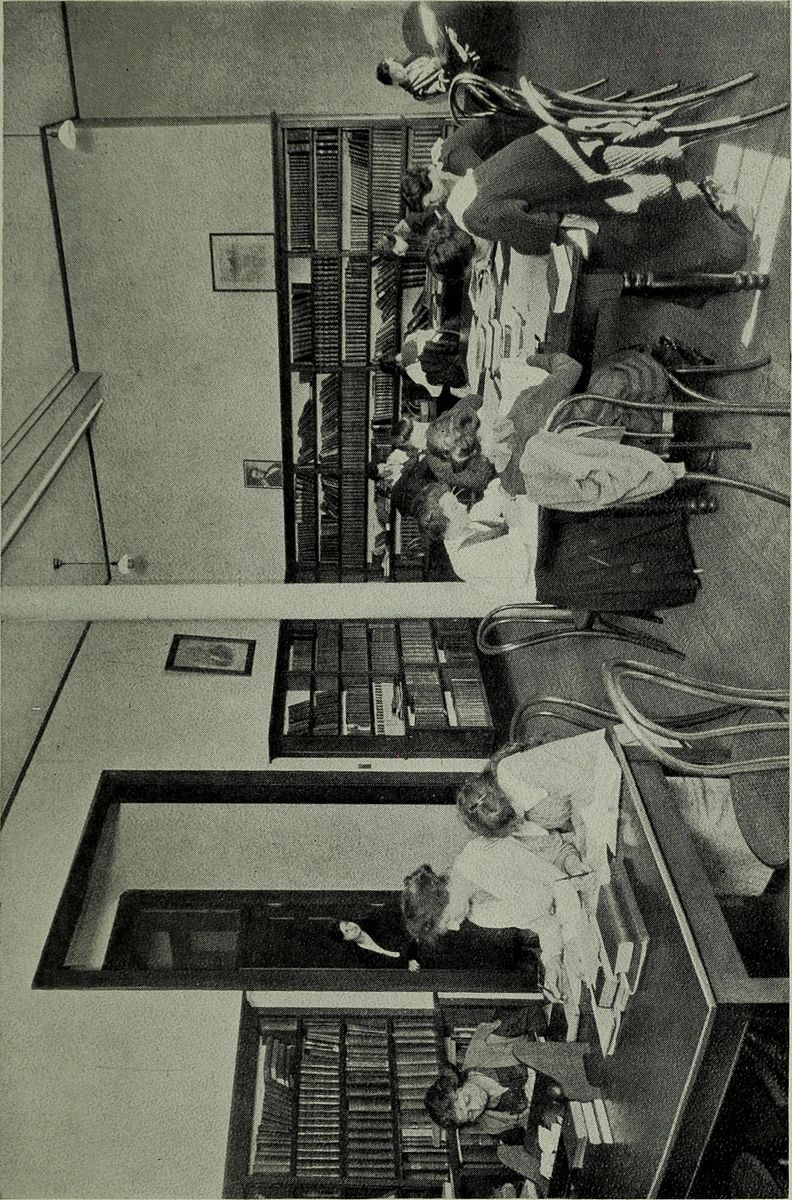
\includegraphics[width=.34\textwidth,angle=-90,trim=0 0 10 10, clip=true]{ladies-hall}
\end{center}
\vspace{-.5cm}
\caption{Queens College, North Carolina. Public
  domain.\label{ladies-hall}}
\vspace{-.3cm}
\end{wrapfigure}

\subsubsection*{Example 2}
Progressive thinkers have for
some time subscribed to the view that ``there shall be no women in
case there be not men, nor men in case there be not women''
\cite[Chapter 1.LII]{rabelais1894gargantua}.
A separate Ladies Hall seems entirely archaic.
However, in light of the
extreme gender imbalance in free software, and still striking
imbalance at Wikipedia \cite{gender,FM4291}, it will be important to
do whatever it takes to make women and girls welcome, not least
because this is a significant factor in boosting our
\patternname{Carrying capacity}.

%\subsubsection*{Summary}

\begin{framed}
\noindent 
\emph{What's Next in the Peeragogy Project}
\definecollection{CarryingWN}
\begin{collectinmacro}{\CarryingWN}{}{}
Making it easy and fruitful for others to get involved is one of the best ways to redistribute the load.  This often requires skill development among those involved; compare the \patternname{Newcomer} pattern.
\end{collectinmacro}
\CarryingWN
\end{framed}



  
